\chapter{Background}

\section{Bitcoin}
The model of traditional banking is based on a centralised trusted authority \cite{RefWorks:doc:5c39e80ae4b0854ae611b047}; we use a third party that we trust in order to mediate the transfer of funds, a process in which we must explicitly define the payee and the payer (i.e. we must identify our friend and ourselves, if we were transferring money to a friend). Bitcoin has no central authority, it is a distributed peer-to-peer system. Therefore, sending money to our friend as before no longer requires any mediation; we send it directly to them. However, transferring funds peer-to-peer of course possesses several challenges; how do you prevent double spending? How do we ensure money is not counterfeit? \cite{RefWorks:doc:5c39e80ae4b0854ae611b047} How is currency issued without a central authority? 
\\\\
Bitcoin solves these challenges by relying on the \textit{Blockchain} [see \ref{background-blockchain}] for its 'source of truth', which itself is secured through \textit{mining} [see \ref{background-mining}] and network-wide consensus \cite{RefWorks:doc:5c39e80ae4b0854ae611b047}. All \textit{transactions} [see \ref{background-transactions}] are publicly available to view on the Blockchain and can be verified by any \textit{node} [see \ref{background-nodes}]. 

\subsection{Addresses, Keys &\& Hashing}
A fundamental concept to Bitcoin is public key cryptography. The basic idea is that we generate a private and public key pair. We can pick a private key at random and use that to generate a public key (using \gls{elliptic-curve-crypto}). The public key can then be used to receive funds [see transactions \ref{background-transactions}] and the private key used to sign transactions to spend the funds. \cite{RefWorks:doc:5c39e80ae4b0854ae611b047}. It is critical to Bitcoin security that the process of generating a public key from a private key is one way and using a public key, it should be impossible to generate the private key. 
\\\\
A Bitcoin address can be generated from a public key. This Bitcoin address is the only information that a user needs to offer in order to receive payments, and since the address essentially appears as random combination of letters and characters, it does not \textit{directly} identify the user which generated the address. However, since all transactions are published publicly, Bitcoin only has pseudo-anonymity [see \ref{background-anonymity}].

\subsection{Blockchain} \label{background-blockchain}
The Blockchain is the global ledger for Bitcoin. It contains the entire Bitcoin history, from the \gls{genesis} to the most recently mined block. It exists as an ordered, back-linked list of blocks of transactions \cite{RefWorks:doc:5c39e80ae4b0854ae611b047} where each block is linked to its previous block, known as its parent block, up to the genesis block. 
\\\\
A block contains a header, containing metadata, then a list of transactions that are included in that block \cite{RefWorks:doc:5c39e80ae4b0854ae611b047} (see figure \ref{fig:simplified-block-structure}). A block can be uniquely identified by a cryptographic hash of its header. The metadata of the block contains data such as the previous block hash (used to create the chain link to the parent described earlier), a difficulty target and the nonce (used in the process of mining explained in \ref{background-proof-of-work}).  

\begin{figure}[h!]
  \centering
  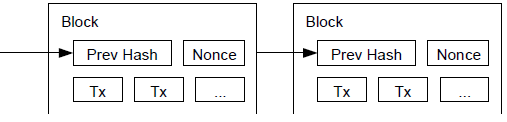
\includegraphics[width = 15cm]{./figures/block-structure-simple}\\[0.5cm] 
  \caption{A simplified block structure. \cite{RefWorks:doc:5c39e80ae4b0854ae611b047}}
  \label{fig:simplified-block-structure}
\end{figure}

\subsection{Mining}\label{background-mining}
Mining is the mechanism that underpins the decentralised clearinghouse of transactions and also the mechanism in which new bitcoin is (currently) issued. Miners, incentivised by the reward of bitcoin, continuously compete to solve the \textit{proof-of-work algorithm} [see \ref{background-proof-of-work}] for each block. 
\\\\
As soon as a miner finds a solution for a block they are mining, they propagate this to the network, allowing each node to independently validate the block. In order to receive compensation for their efforts, a miner must include in the block a special transaction from the \textit{coinbase} [see \ref{background-coinbase}] to their own public address. If the block is valid, then the block will be added to the blockchain and eventually the miner will be remunerated with new bitcoin from the coinbase. The successful miner also claims the transaction fees for the transactions included in the mined block. For all nodes that see this newly mined block, and is part of their longest chain, the next round of mining begins immediately, again competing to find the solution of the next blocks proof-of-work algorithm. 

\subsection{Coinbase}\label{background-coinbase}
The coinbase refers to the input of a special type of transaction (the coinbase transaction) which, unlike regular transactions, does not consume bitcoin (i.e. it has no 'spending element'). Rather, it has a singular input called the \textit{coinbase}. The bitcoin is therefore created out of nothing. This is the mechanism in which new bitcoin are introduced into the network. 

\subsection{Proof of work}\label{background-proof-of-work}
New blocks are mined approximately every 10 minutes; this rate of mining is maintained even with fluctuations in the hash-rate of the network by periodically adjusting the difficulty of the proof-of-work algorithm. A change in hash-rate can be attributed to an increased/reduced amount of computational power of the network; this can be caused by a change in the number of participants or advancements in mining hardware.
\\\\
As shown in figure \ref{fig:all-time-hash-rate} the hash-rate of Bitcoin has grown exponentially in recent years, reflecting an increase in the number of nodes in addition to advances in hardware. There is, however, a noticeable decline in hash-rate quite recently (around the time of November 2018) due to a \textit{hard-fork} [see \ref{background-forks}]. Comparing the hash-rate to difficulty over time (see figure \ref{fig:all-time-difficulty}) demonstrates how Bitcoin's difficulty is dynamically adjusted in response to changes in the networks hash-rate. 
\\\\
So, what exactly is the proof-of-work algorithm that miners are trying to solve? Firstly, observe in figure \ref{fig:simplified-block-structure} there exists a 'nonce' field. This exists as a variable that can be changed freely by a miner. As simply put as possible, the miner wants to find a hash for the block that is lower than some target value. This is achieved by repeatedly adjusting the nonce field and generating the new resulting block hash and comparing it to the target. Since a hash function is one-way, we have the property that a miner can only find a hash lower than the target is by performing repeated trial and error of nonce's/hashes (i.e iterating through different values for the nonce and looking at the hash of the block with that nonce value).
\\\\
Clearly, the problem of finding a hash lower than a target can have its difficulty adjusted by adjusting how small or large the target is. A lower target will have less hashes that are smaller than it, and therefore a lower probability of finding a satisfying hash; the difficulty and the target are inversely related. 
\\\\
In summary, the Proof-of-Work problem creates measure of computational effort that must have been spent in order to achieve a valid solution. Although it is theoretically possible to find a satisfying solution immediately, it is incredibly unlikely and by adjusting difficulty accordingly, Bitcoin achieves an average of ~10 minutes' worth of the networks computational effort being spent for each solution that is found. 


\begin{figure}[h!]
  \centering
  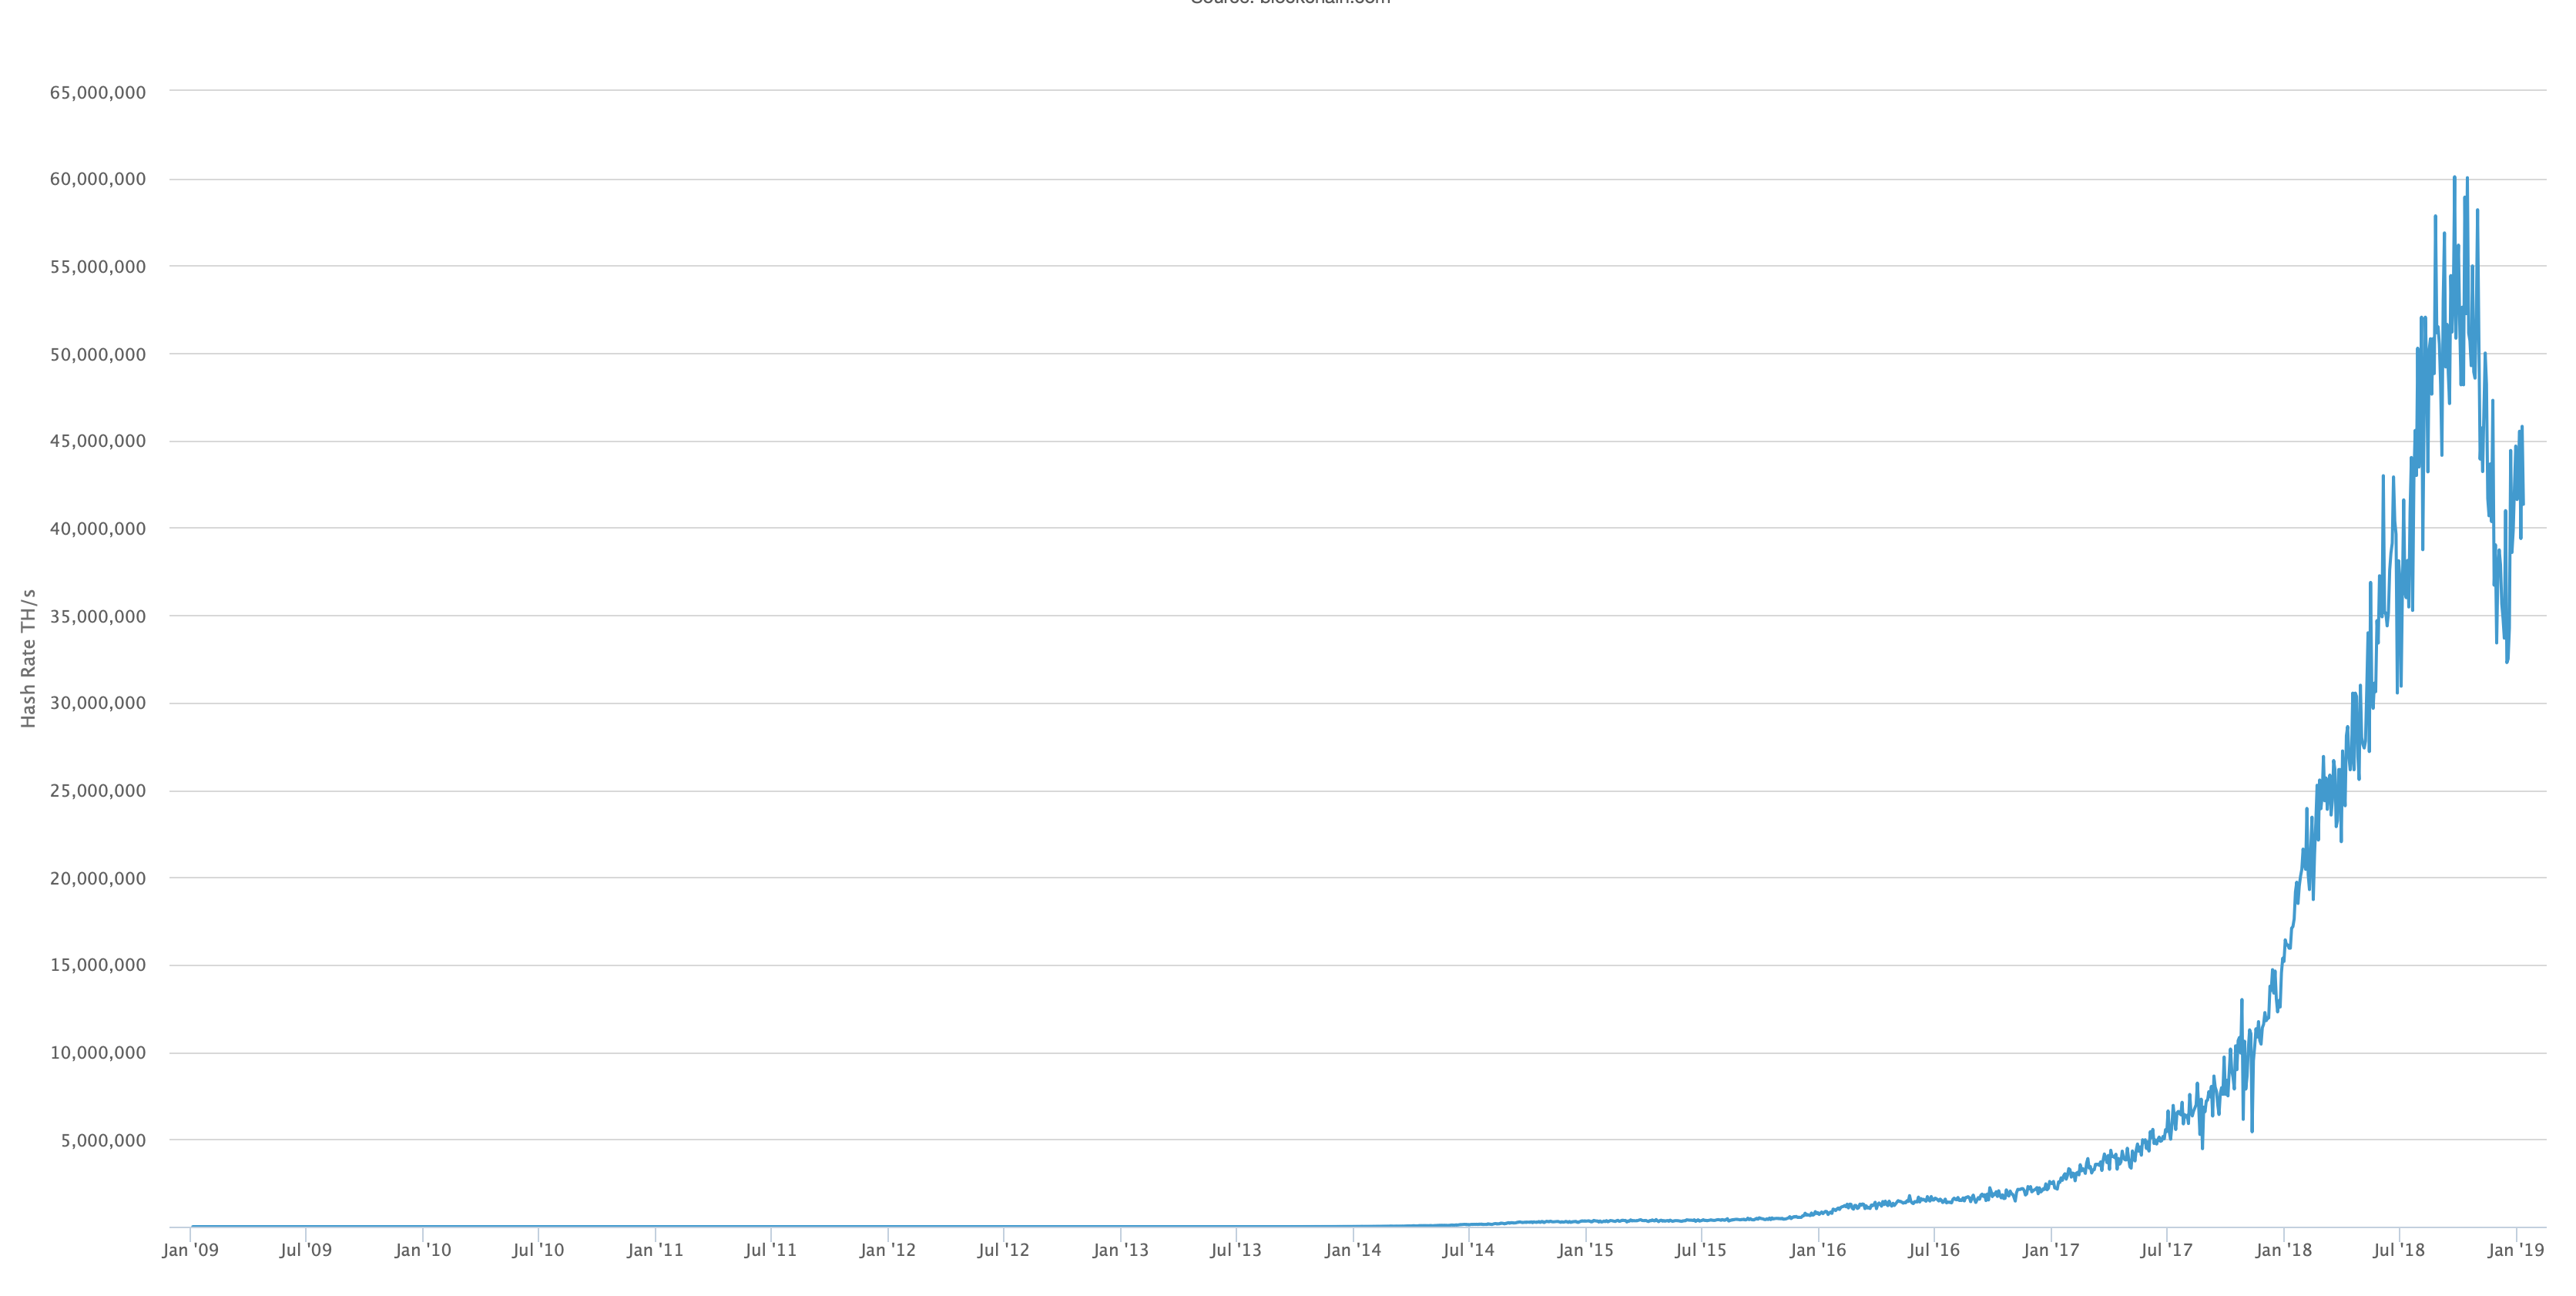
\includegraphics[width = 15cm]{./figures/hashrate-all-time}\\[0.5cm] 
  \caption{Bitcoin hash-rate for all of time. \cite{RefWorks:doc:5c3b0c9de4b066461b1b87bb}}
  \label{fig:all-time-hash-rate}
\end{figure}

\begin{figure}[h!]
  \centering
  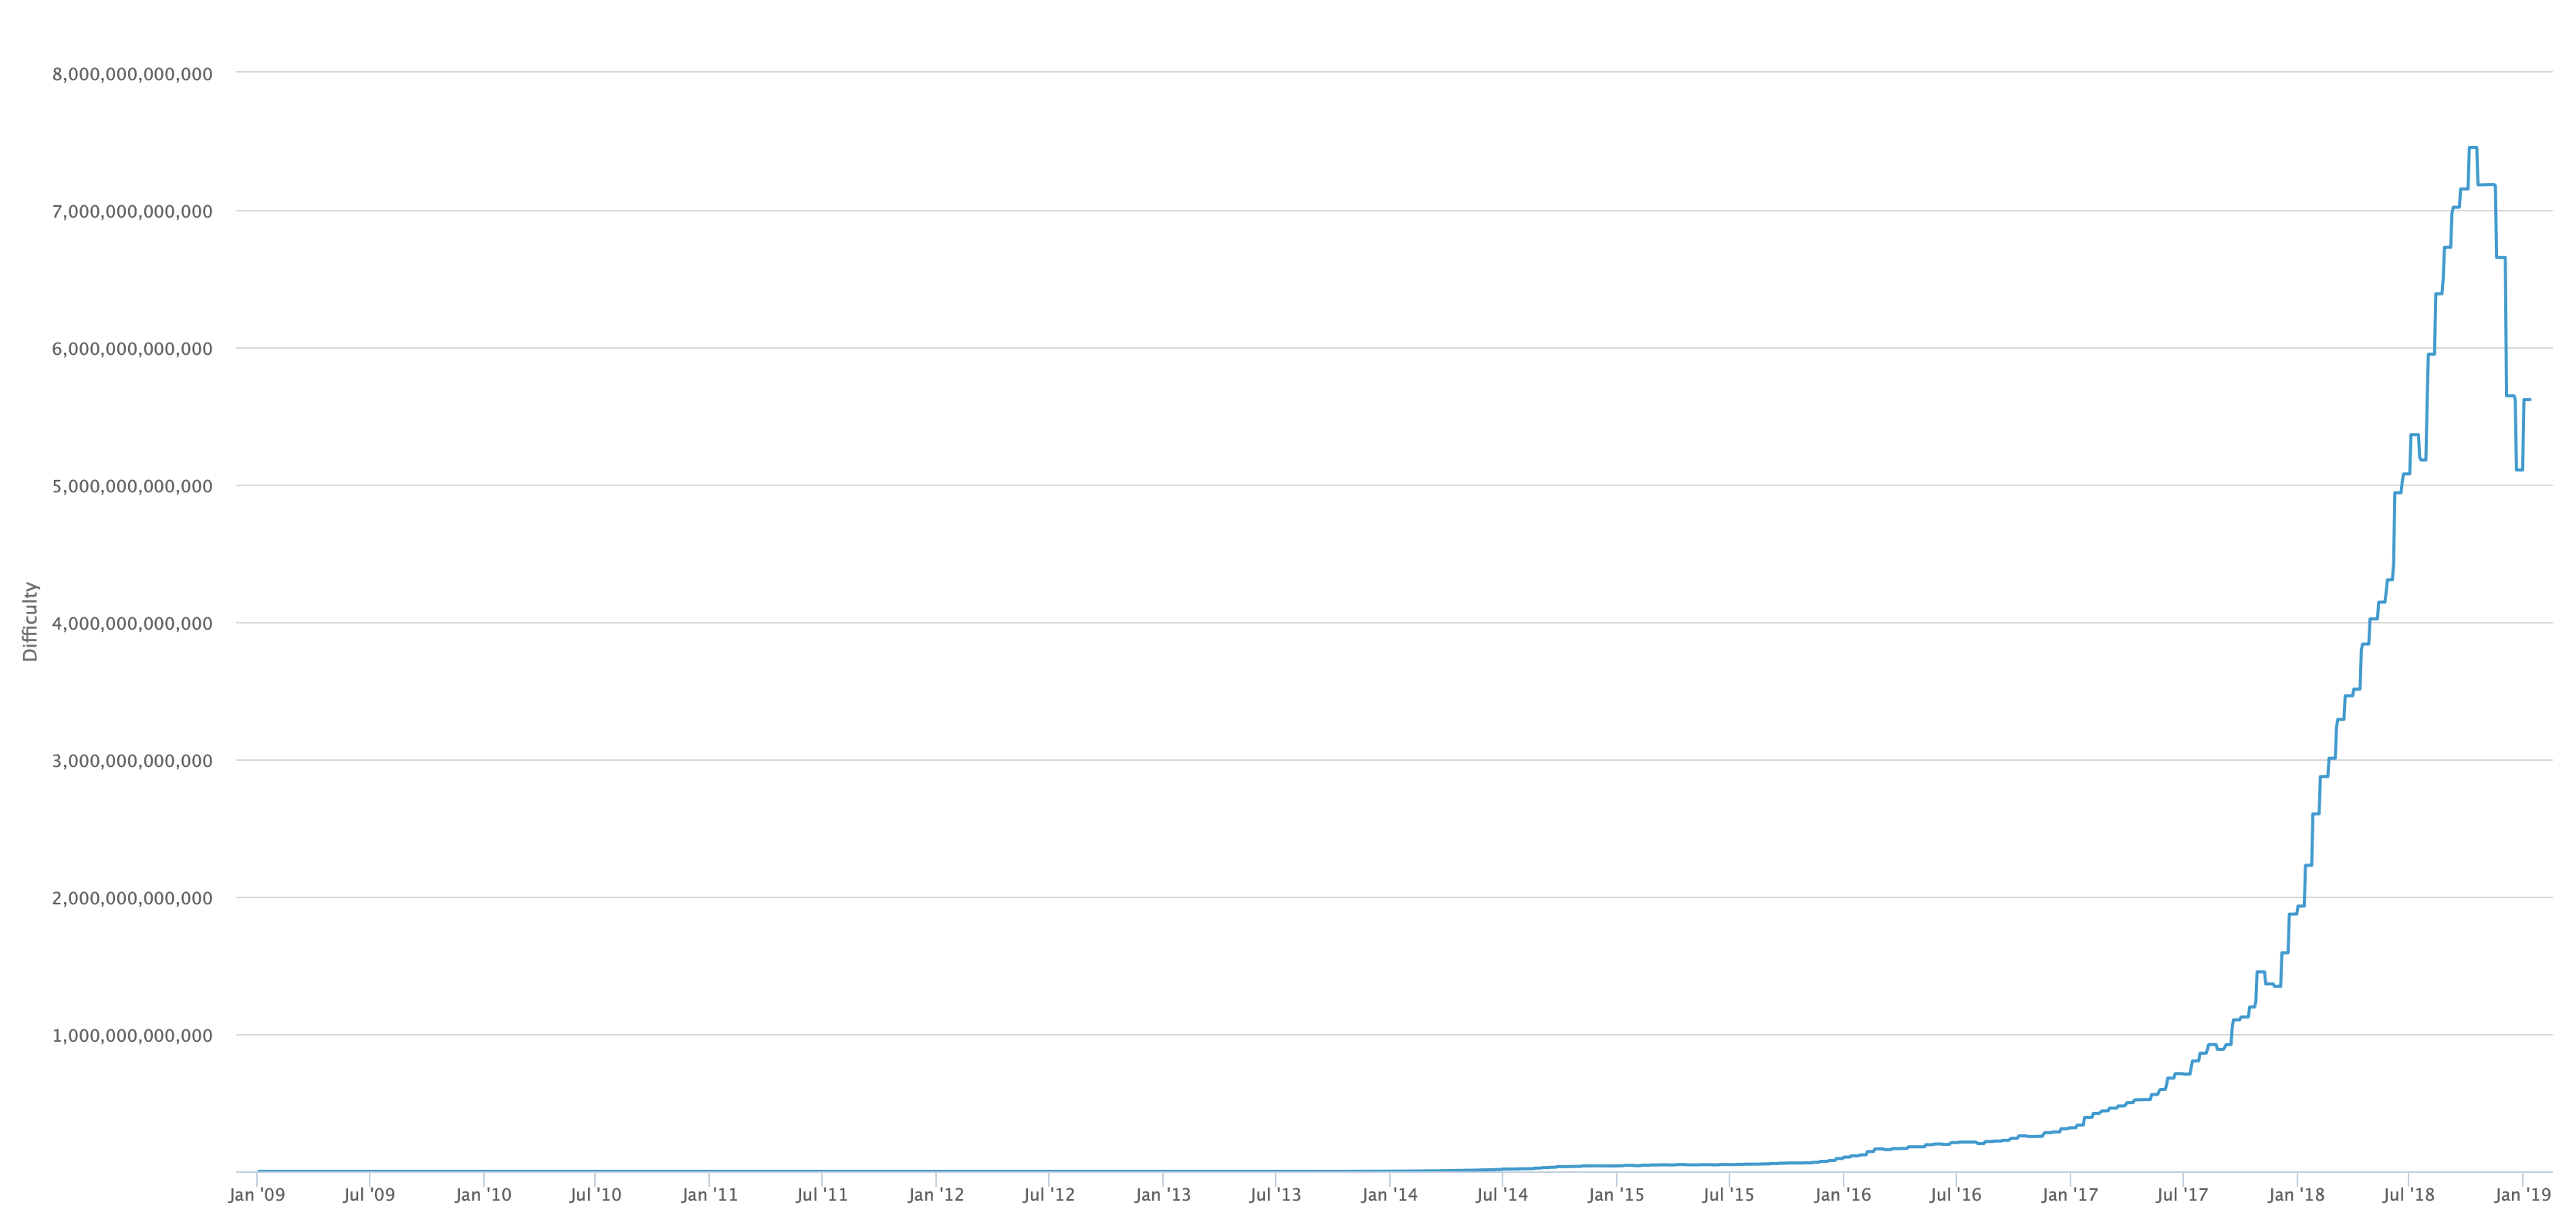
\includegraphics[width = 15cm]{./figures/difficulty-all-time}\\[0.5cm] 
  \caption{Bitcoin difficulty for all of time. \cite{RefWorks:doc:5c3b1ac4e4b0ea619644bcc1}}
  \label{fig:all-time-difficulty}
\end{figure}


\subsection{Transactions}\label{background-transactions}
Transactions are the core component facilitating the transfer of funds in Bitcoin. A transaction tells the network that the owner of some bitcoin value has authorised the transfer of that value to another owner \cite{RefWorks:doc:5c39e80ae4b0854ae611b047}. In the simplest case, transactions contain inputs, which represent where the funds are coming from (the sender), and outputs, which represent where the funds are going to (the new owner). 
\\\\
For the transfer of funds to be confirmed, the transaction must be added to the global ledger for everyone to see. This means it must be included in a block that is mined on the Blockchain. To be included in a future block, the transaction must be propagated to the many nodes of the network. The creator of the transaction must therefore send it to some of the Bitcoin nodes it knows the location of (its neighbours). These nodes, if the transaction is valid, will propagate the transaction to their neighbours, which will repeat the same process. This is the process of 'flooding' the network with the transaction. In addition to sending the bitcoin value to the recipient, the sender must also include an incentive for the miner to perform the work to include the transaction in the block they are currently mining. This is the \textit{transaction fee}.
\\\\
The transaction fee is a small value that is implicitly included in the transaction by leaving some left-over funds from the inputs once the recipient of the transaction has been 'paid'. This fee is collected by the miner who includes the transaction in the block they mined. A larger fee will act as a higher incentive for a miner to include the transaction in the block and will likely result in the transaction being included in the Blockchain in a timelier fashion.  

\subsection{Nodes}\label{background-nodes}
There are several different types of nodes in Bitcoin. One type of node is the 'full node'. Full nodes nodes maintain a copy of the entire Blockchain locally, containing all transactions. These nodes must maintain and build their copy of the Blockchain by listening to incoming transactions and blocks. A full node can independently verify each transaction and block using its own copy of the Blockchain, without relying on information from other nodes. The disadvantage of running a full node is that it consumes a large amount of storage. 
\\\\
Not all nodes require a full copy of the Blockchain, and in many cases cannot hold a full copy due to resource constraints on devices such as smart-phones. These nodes are called Simplified Payment Verification (SPV)\cite{RefWorks:doc:5c39e80ae4b0854ae611b047} nodes. These nodes do not have a full picture of the history of Bitcoin (i.e all of the transactions) but do know all of the hashes of the blocks in the Blockchain. A SPV node therefore uses the depth of the block that the transaction is in to verify it, in comparison to the full node which will build a full database of unspent bitcoin from the transaction to the genesis block and verify it is not a double spend. The SPV node will wait until the transaction is in a block at depth of at least 6, relying on the knowledge that other nodes have accepted the transaction as confirmation that the transaction is valid. 

\subsection{Immutable History}
The Blockchain ledger becomes more and more immutable as time passes; this is because in order to add a different block into the Blockchain, you must expend effort to re-do the proof-of-work for that block. Then, in order to change a block buried under other blocks, you must also expend the energy to re-do the proof-of-work for all of the blocks it is buried under (since you now require a different parent block hash field value and will then get a different hash for child blocks). This makes it exponentially less likely to be able to catch up with the main chain as the chain grows \cite{RefWorks:doc:5c3b547fe4b0613d0cda0434}. Therefore, the more blocks a block is 'buried' by, the more immutable it becomes, making old blocks in the chain are practically immutable \cite{RefWorks:doc:5c39e80ae4b0854ae611b047}. 



\subsection{Mining Pools}
As touched upon earlier in mining [see \ref{background-mining}], a miner must expend enormous amounts of energy/ computational effort in order to compete for the proof-of-work solution of a block, resulting in them being compensated for their efforts with new bitcoin. 
\\\\
A miner without a huge amount of resources at their disposal (i.e. warehouses of machines) will find it very unlikely to successfully mine a block and be compensated for their efforts. It may be the case that they must mine for years before they are successful. This makes investing in hardware and energy too much of a gamble for most, and they will likely seek more frequent enumeration for their efforts. Allowing for more frequent enumeration for computation efforts is the purpose of mining pools.
\\\\
Mining pools essentially pool many miners' resources in order to mine a block. Using many participants, a pool will have a much higher likelihood of being successful in mining a block. The reward of bitcoin is then paid to the pool, which the pool then distributed amongst the contributing members of the pool. A pool measures contributions of miners by giving the miners a much lower target for the block they are mining than the actual, more difficult, Bitcoin target. This will allow miners to successfully mine their blocks with the lower target far more often, which the pool can recognise and use this as a measure of their contribution. Every now and then, a pool miner will mine a block that is lower than the pool target and lower than the Bitcoin target, which the pool will use as the overall succeeding block and propagate to the network.

\subsection{Forks}\label{background-forks}
A fork on the Blockchain can occur naturally, an inherent property of a decentralised network such as Bitcoin is that different nodes can have different views of the world (i.e. due to transmission delays)- however these forks are usually quickly corrected within a small number of (usually one) blocks \cite{RefWorks:doc:5c39e80ae4b0854ae611b047}. There also exist forks that have been deliberately created, i.e. by an attacker attempting to re-write history of the Blockchain, or by a \textit{hard-fork} software release. 
\\\\
A hard-fork in the Blockchain is where the Bitcoin network permanently diverges. A hard-fork occurs when there is a change in the consensus rules. The consensus rules tell a node which blocks to accept, and which ones to reject. A block must conform to the consensus rules of the majority of nodes in order to be added to the chain. When a change to consensus rules occurs, not all nodes may be on-board. Some may still be running with the old consensus rules. This would mean they would create and accept blocks using the old rules rather than the new ones - meaning their blocks will not be accepted by nodes running with the new rules (hard-forks mean a non-backwards compatible change). This leads to a divergence in the chain, where one chain is based on blocks added by nodes running the old rules, and the other chain containing blocks added by nodes running with the new rules. 
\\\\
In a similar vein, there also exist 'soft forks' which do not lead to a divergence of the Blockchain since they incorporate a backwards-compatible change. This means that blocks added by nodes running the old software will not be rejected by those running the new software. 
\\\\
Figure \ref{fig:hard-fork} shows how a hard-fork will look on the Blockchain; the fork at block 3 represents a naturally occurring fork as mentioned at the beginning of this section, whereas the fork occurring at block 6 is a hard-fork and may be due to a change in the consensus rules of the network \cite{RefWorks:doc:5c39e80ae4b0854ae611b047}. 

\begin{figure}[h!]
  \centering
  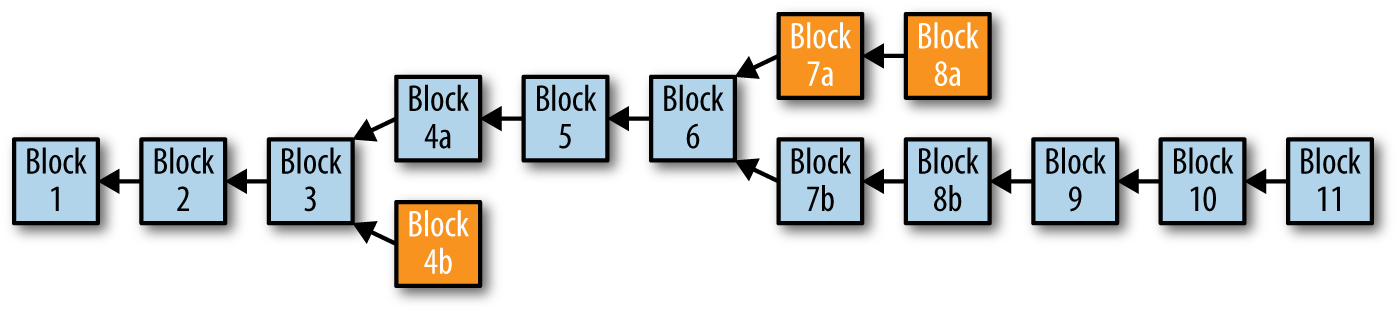
\includegraphics[width = 15cm]{./figures/hard-fork}\\[0.5cm] 
  \caption{An example of a hard-fork. \cite{RefWorks:doc:5c39e80ae4b0854ae611b047}}
  \label{fig:hard-fork}
\end{figure}


\section{Anonymity}\label{background-anonymity}

Since all transactions to occur in Bitcoin are available to view by the public, Bitcoin can only offer pseudo-anonymity rather than real anonymity \cite{RefWorks:doc:5c3db7d6e4b0fa2b1fe68b48}.

There exist studies which show it is possible to de-anonymise Bitcoin transactions based on data that is publicly available \cite{RefWorks:doc:5c3db7d6e4b0fa2b1fe68b48}. Therefore, there exist services called 'mixers' which aim to obfuscate transaction origins and make the de-anonymisation of Bitcoin transactions more difficult. 

\subsection{Mixing Services}\label{background-mixing-service}
A mixing service, or 'mixer', works in the following way: A user wishing to user a mixing service will first create a new address and send bitcoin to an address of the service, asking the service to send the funds back to their new address. Other users also wishing to achieve the same goal will take the same steps and send bitcoin to the service. The service now holds bitcoin for multiple users. The service can now use any of the addresses in which it holds bitcoin to send money back to the users of the service. This results in the appearance of a disconnect between the user's old address (the one which held the bitcoin initially) and the new address which now holds their bitcoin \cite{RefWorks:doc:5c3dace5e4b0613d0cda512b}. Clearly, this helps disguise the origins of bitcoin, and can be used as a tool in the process of money laundering. The operators of these services profit by charging a fee in exchange for 'mixing' their bitcoin. 

\subsection{Attacks on transactions anonymisers}
In order for a mixing service to provide functionality, it will likely retain a history of the senders and recipients. If an attacker wishing to discover users using these services were to setup a Mixer, they could potentially gain a full knowledge of relationships between senders and recipients if logs were to be kept for this data over a large enough time span \cite{RefWorks:doc:5c3dace5e4b0613d0cda512b}. Of course, this would only be effective if the user were to rely on a single mixing service and could mitigate this vulnerability by using multiple mixing services, but at the cost of paying more fees. 
\\\\
Other weaknesses in anonymisation services could be the timing of incoming and outgoing transactions, in addition to transaction values, which could all be used to correlate the senders and recipients of bitcoin. Furthermore, the communication between the user and the service itself, if compromised, could reveal information (such as addresses) used to de-anonymise transactions. 
\\\\
In addition, studies have shown other mixing services such as Bitlaunder, DarkLaunder and Coinmixer have multiple serious security flaws and can be quite easily attacked to compromise the privacy of those that use it. In fact, the investigation shows that making a mixer that is genuinely secure is far from an easy task, which may be refreshing news for law enforcement wishing to taint bitcoin back to its source, but worry-some for legitimate users of such mixing services \cite{RefWorks:doc:5c3db214e4b0854ae6124c26}. 


\subsection{Peeling Chain}\label{background-peeling-chain}
A peeling chain is a pattern of use that exists widely in the Bitcoin network; it can be used in withdrawals from exchange services, mining pools and potentially in use cases related to criminal activity. The chain begins at an address that often holds a large bitcoin value, and the goal is to obfuscate the funds that a wallet holds. This is achieved by a series of transactions in which the bitcoin will be sent to two or more addresses, one of which will belong to the service (which owns the originating address) where the majority of the bitcoin will be sent, and the small remainder to some change addresses. 
\\\\
Recently, peel chains are being used less frequently due to modern Blockchain analysis software developing the capability to collapse even the most complex peel chains. There also exists transaction fees at each hop of the peel chain, so they are increasingly becoming less attractive. 
\begin{figure}[h!]
  \centering
  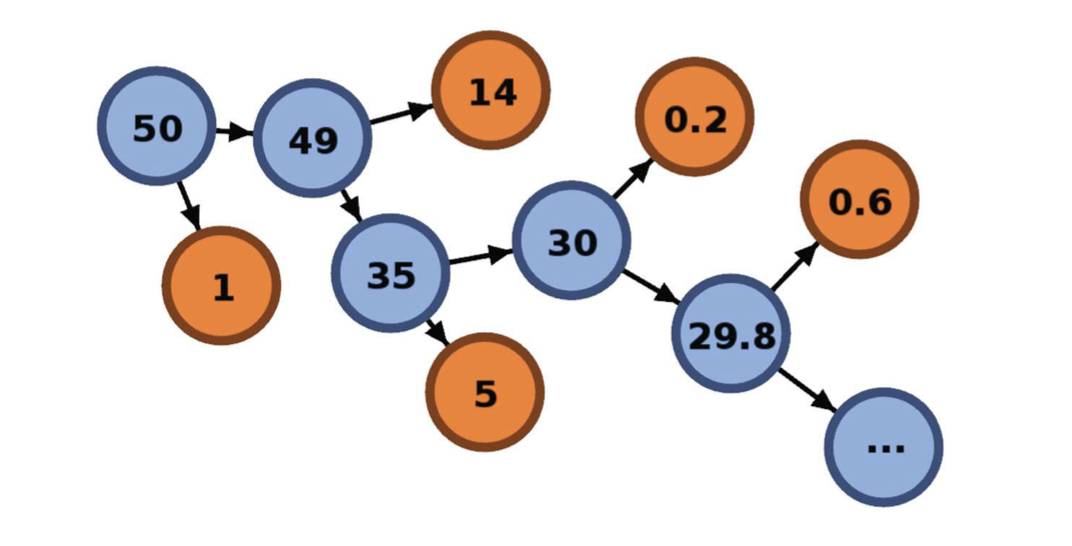
\includegraphics[width = 10cm]{./figures/peel-chain}\\[0.5cm] 
  \caption{An example of a peel chain. \cite{RefWorks:doc:5c3db214e4b0854ae6124c26}}
  \label{fig:peel-chain}
\end{figure}


\subsection{Taint Analysis}\label{background-taint}
Taint analysis was a service that was offered free by blockchain.info which aims to calculate the correlation between two addresses. The definition on the site was \lq Taint is the \% of funds received by an address that can be traced back to another address\rq. The taint therefore usually correlates with the percentage of funds that are linked to some theft of coins, or are known to have been used in some illicit manner. However, this feature is no longer available on the site, with some speculation to the feature being retracted in order to provide it as a charged, premium offering. 

\subsection{Tor}
The onion router (tor) is an infrastructure for providing private communication over a public network. In onion routing, instead of making connections directly with a machine you'd like to communicate with, you make connections through a sequence machines called onion routers. These routers will be typically located across the glove. Messages are sent in multiple layers of encryption for each relay, so each relay can decrypt the outer layer and forward the decrypted resulting message onto the next router. Eventually, the one-layer encrypted message will reach its destination. Using Tor therefore permits for protection against eavesdropping and traffic analysis \cite{RefWorks:doc:5c3e103be4b014f3944e4192}.

\section{Bitcoin address clustering (on-chain)}

It is possible to define a number of heuristics that can be used in an effort to group distinct Bitcoin addresses so that they can be collectively associated with individual user. This section outlines some of these heuristics that use data from the Blockchain to help cluster addresses belonging to the same user.

\subsection{Multi-input transactions}\label{background:multi-input-tx}
Multi-input transactions will be required when some user, say Alice, wishes to transfer some funds, say the value of $v$ to some other user Bob; however, Alice does not hold a single bitcoin denomination that is greater or equal to $v$ and therefore must combine multiple smaller denominations to meet/exceed the value of $v$. It is therefore relatively trivial to conclude by inspecting the inputs of these transactions, that the addresses of each of the inputs are in-fact owned by the same user Alice \cite{RefWorks:doc:5c3de14be4b042abd3bcc2c6}.

\subsection{Change Addresses}
A transaction will also often generate change, where the value of the inputs exceeds the amount to be paid to the recipient and any transaction fees, and the remainder will want to be paid back to the sender. To do this, Bitcoin will generate a change address for the remainder to be sent to. Therefore, it can usually be safely assumed that when a transaction has two outputs, and one is a new address that has not appeared before, that this address is the change address and belongs to the sender of bitcoin for this transaction \cite{RefWorks:doc:5c3de14be4b042abd3bcc2c6}. 
\\\\
A weakness in using this heuristic as highlighted in previous research \cite{Refworks:doc:5c3de7e3e4b0ea6196452d80} is that it is not robust in the face of changing patterns of use in the network since it is an idiom of use rather than an inherent property of Bitcoin. In fact, the study in \lq A fistful of Bitcoins\rq  \cite{Refworks:doc:5c3de7e3e4b0ea6196452d80} found that falsely linking just a small number of change addresses causes entire relationship graphs to collapse into giant clusters that are not actually controlled by a single user. 
\\\\
However, through careful investigation of false positives and making the algorithm for change address clustering more conservative, the team from \lq A fistful of Bitcoins\rq were able to name 1,600 times more addresses post-clustering than they already knew the identify of (through hand tagging) \cite{Refworks:doc:5c3de7e3e4b0ea6196452d80}. Evidently, these heuristics could be extremely useful in the process of identifying users and tracking funds, such as by collapsing peeling chains [see peeling chain \ref{background-peeling-chain}].

\subsection{Behaviour based analysis}
Humans naturally fall exhibit behaviour patterns, and since many events on the Blockchain are human driven, it is possible to attempt to identify these behaviour patterns and apply them in clustering the activities of distinct users. Using timestamps and network properties, it becomes possible to observe such behaviour patterns could include items being purchased, daily schedule and activities, in addition to non-human behaviour patterns of hardware and network latencies \cite{RefWorks:doc:5c3f3459e4b042abd3bceede}. 
\\\\
The study 'Identifying Bitcoin users by transaction behaviour' \cite{RefWorks:doc:5c3f3459e4b042abd3bceede} shows that a transaction can be described by its timestamp, connectivity (number of inputs/outputs) and coin flow. From these transactions, features can be extracted that help characterise some aspect of transaction behaviour over time. These features are: 
\begin{itemize}
    \item The time interval between successive transactions
    \item The hour of day the transaction took place
    \item The time of hour (seconds since start of hour)
    \item The time of day (seconds since start of day)
    \item Coin flow - the net bitcoin value  
    \item Input/output balance - The balance of inputs from other users compared to outputs going to other users.
\end{itemize}


\section{Bitcoin address clustering (off-chain)}
The previous section outlines heuristics for using on-chain data for address clustering, however it is possible that there exists more public information available elsewhere on the internet that can be used to help cluster addresses \cite{RefWorks:doc:5c3ef27be4b03c7dd82ce4e6}. 

\subsection{Tag Collection}\label{background-tag-collection}
Tag collection is the process of trying to find a Bitcoin address that is mentioned in the same data frame as some tag (such as a username or a company name) \cite{RefWorks:doc:5c3ef27be4b03c7dd82ce4e6}. Therefore, passive tag collection can be carried out by crawling sites where this information is likely to appear, such as social media, bitcoin forums and dark-web marketplaces (for example, Silkroad). Tagging in this manner may allow addresses to be correlated to known Bitcoin businesses, or categorised in the type of service they are, such as an exchange, marketplace, mining pool, mixer, gambling etc. 


\section{Popular Services}
\subsection{Satoshi Dice}
A very popular Bitcoin dice game, introduced in April 2012, is Satoshi Dice. Users may place bets and, if they win, have some multiple of their bets paid back to them \cite{Refworks:doc:5c3de7e3e4b0ea6196452d80}. It is estimated that Satoshi Dice is responsible for about 60\% of activity on the Bitcoin network and is expected to contribute an extra 14MB to the overall Blockchain daily \cite{Refworks:doc:5c3de7e3e4b0ea6196452d80}. 


\subsection{Exchanges}
Often it is unavoidable to use an exchange service. Exchange services enable a user to exchange their currency, such as a \gls{fiat-money} or another cryptocurrency, into bitcoin and vice versa. For those users attempting to user bitcoin for illicit means, this poses an issue as it is a point of centralisation; an example is a user who has stolen bitcoin, who wishes to then convert stolen funds to their fiat currency, but first must go through a known exchange. It's possible their bitcoin is now tainted [see \ref{background-taint}] and will not be accepted by many exchanges. 

\section{Illegal Activity}

The impact Bitcoin can have in facilitating illegal activity is substantial; in a 2012 intelligence report \cite{RefWorks:doc:5c4ad055e4b0ea619646c15a}, the FBI claimed: 

\begin{displayquote}
 ``If Bitcoin stabilizes and grows in popularity, it will become an increasingly useful tool for various illegal activities beyond the cyber realm. For instance, child pornography and Internet gambling are illegal activities already taking place on the Internet which require simple payment transfers. Bitcoin might logically attract money launderers, human traffickers, terrorists, and other criminals who avoid traditional financial systems by using the Internet to conduct global monetary transfers.''
\end{displayquote}

The report now 7 years ago feels almost like an early warning call; since then we have seen the FBI's predictions materialise as we see high-profile thefts, money laundering and drug-buying stories hit headlines. 
\\\\
Why does Bitcoin make life difficult for law enforcement? Bitcoins decentralised nature introduces a number of vulnerabilities to the traditional law enforcement techniques. There is a lack of anti money-laundering software, account owners often cannot be directly identified and it is more difficult to identify the original source of funds \cite{RefWorks:doc:5c4ad055e4b0ea619646c15a}. 

\subsection{Silk Road}
Silk road was an international online marketplace which operates as a Tor hidden service that was overwhelmingly used as a market for controlled substances and narcotics \cite{RefWorks:doc:5c3e0105e4b0854ae612621e}. Through investigation by Nicolas Christin \cite{RefWorks:doc:5c3e0105e4b0854ae612621e}, it appeared to be quite an advanced marketplace including features for a product rating system with customer feedback, an escrow account for dispute management, automatic price pegging to the USD for sellers (automatically accounting for bitcoin price fluctuations) and site-wide promotional campaigns such as 'pot day' \cite{RefWorks:doc:5c3e0105e4b0854ae612621e}. However, in 2013 the FBI shut down Silk road, but an almost identical site Silk Road 2.0 quickly emerged, and began generating sales of \$8 million a month with 150,000 active users. Just a year later, the FBI also shut down Silk Road 2.0 and arrested it's operator \cite{RefWorks:doc:5c4ae400e4b0613d0cdbb201}. 

\subsection{Bitcoin ATM's}

Bitcoin ATM's are physical machines, often installed in small shops, that allow users to buy and sell various cryptocurrencies by trading in their \gls{fiat-money}. For example, there exist many Bitcoin ATM's in London, UK where you buy bitcoin in exchange for depositing pound sterling. The owners of these machines have the incentive of hosting them in their stores as they can charge a commission fee on these transactions. Over the last few years, these ATM's have become increasingly abundant across the UK, as shown in figure \ref{fig:background-atm-growth}. 
\\\\
However, there have been growing concerns that these ATM's are being used in the process of \gls{money-laundering} [see \ref{background-money-laundering}]. In a December 2018 report by Bloomberg \cite{RefWorks:doc:5c4af4bfe4b0686b56fa4839}, reporters carry out an experimental investigation into the counter money-laundering measures being taken by Bitcoin ATM's; estimating that more than half of the machines in the US are not following the rules. Many machines do not verify identification or impose limits on transactions, in direct violation of several US banking laws \cite{RefWorks:doc:5c4af4bfe4b0686b56fa4839}. 

\begin{figure}[h!]
  \centering
  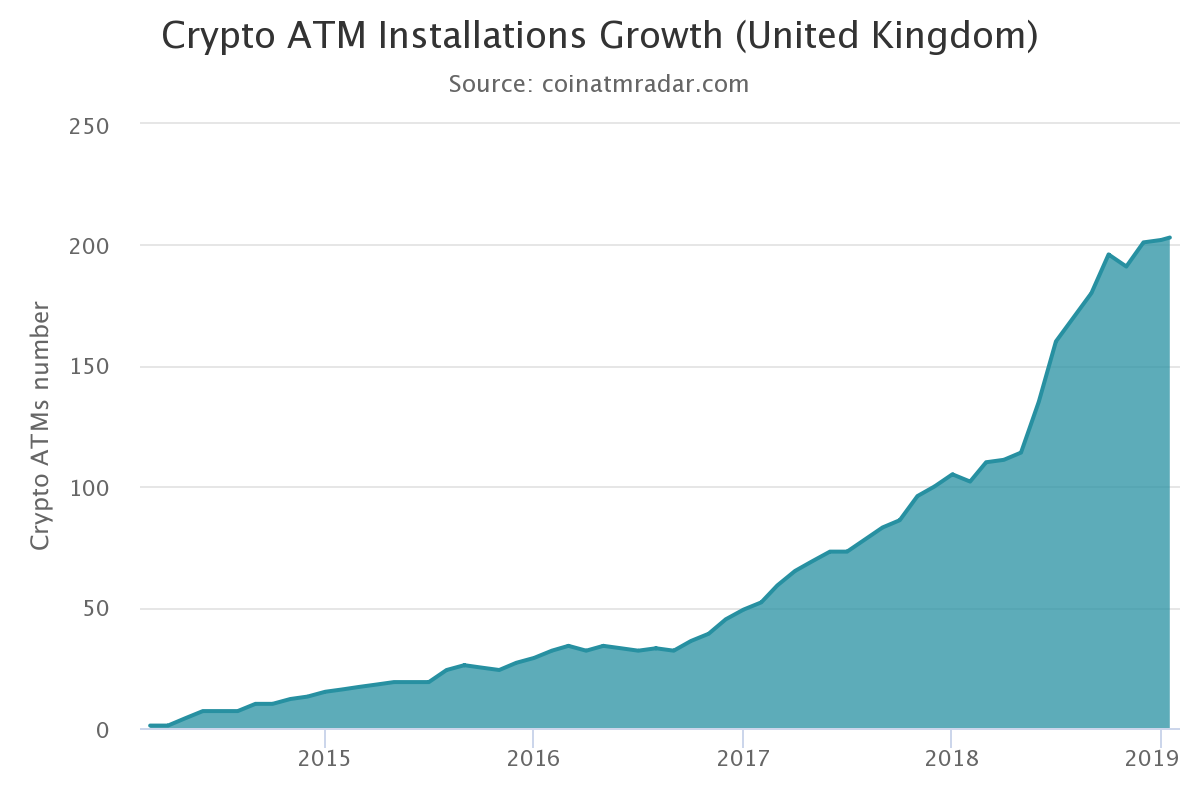
\includegraphics[width = 15cm]{./figures/atm-installs-uk}\\[0.5cm] 
  \caption{Accumulated number of crypto ATMs installed over time - UK only \cite{RefWorks:doc:5c3f53f3e4b029cf9278c787}.}
  \label{fig:background-atm-growth}
\end{figure}


\section{Existing Forensic Tools}\label{background-existing-tools}

The idea of visualising Blockchain data in a graphical, interactive fashion and providing tools for forensics has not been coined by this project. There exist tools, both freely available and proprietary, that aim to deliver similar capabilities. 

\subsection{Blockchain Explorer}
Blockchain Explorer, accessible at https://www.blockchain.com/explorer, provides a wealth of information (available on the blockchain) about addresses, transactions and blocks. For instance users can search by a public address in order to inspect the transactions associated with it. It also has features to provide charts on Bitcoin statistics, such as the network hash rate and exchange rates. However, in order to carry out a forensics investigation, it will often be necessary to follow the path of funds between addresses and simplified by doing this in a graphical way; these are features not provided by Blockchain Explorer, only one address can be viewed at a time. 

\begin{figure}[h!]
  \centering
  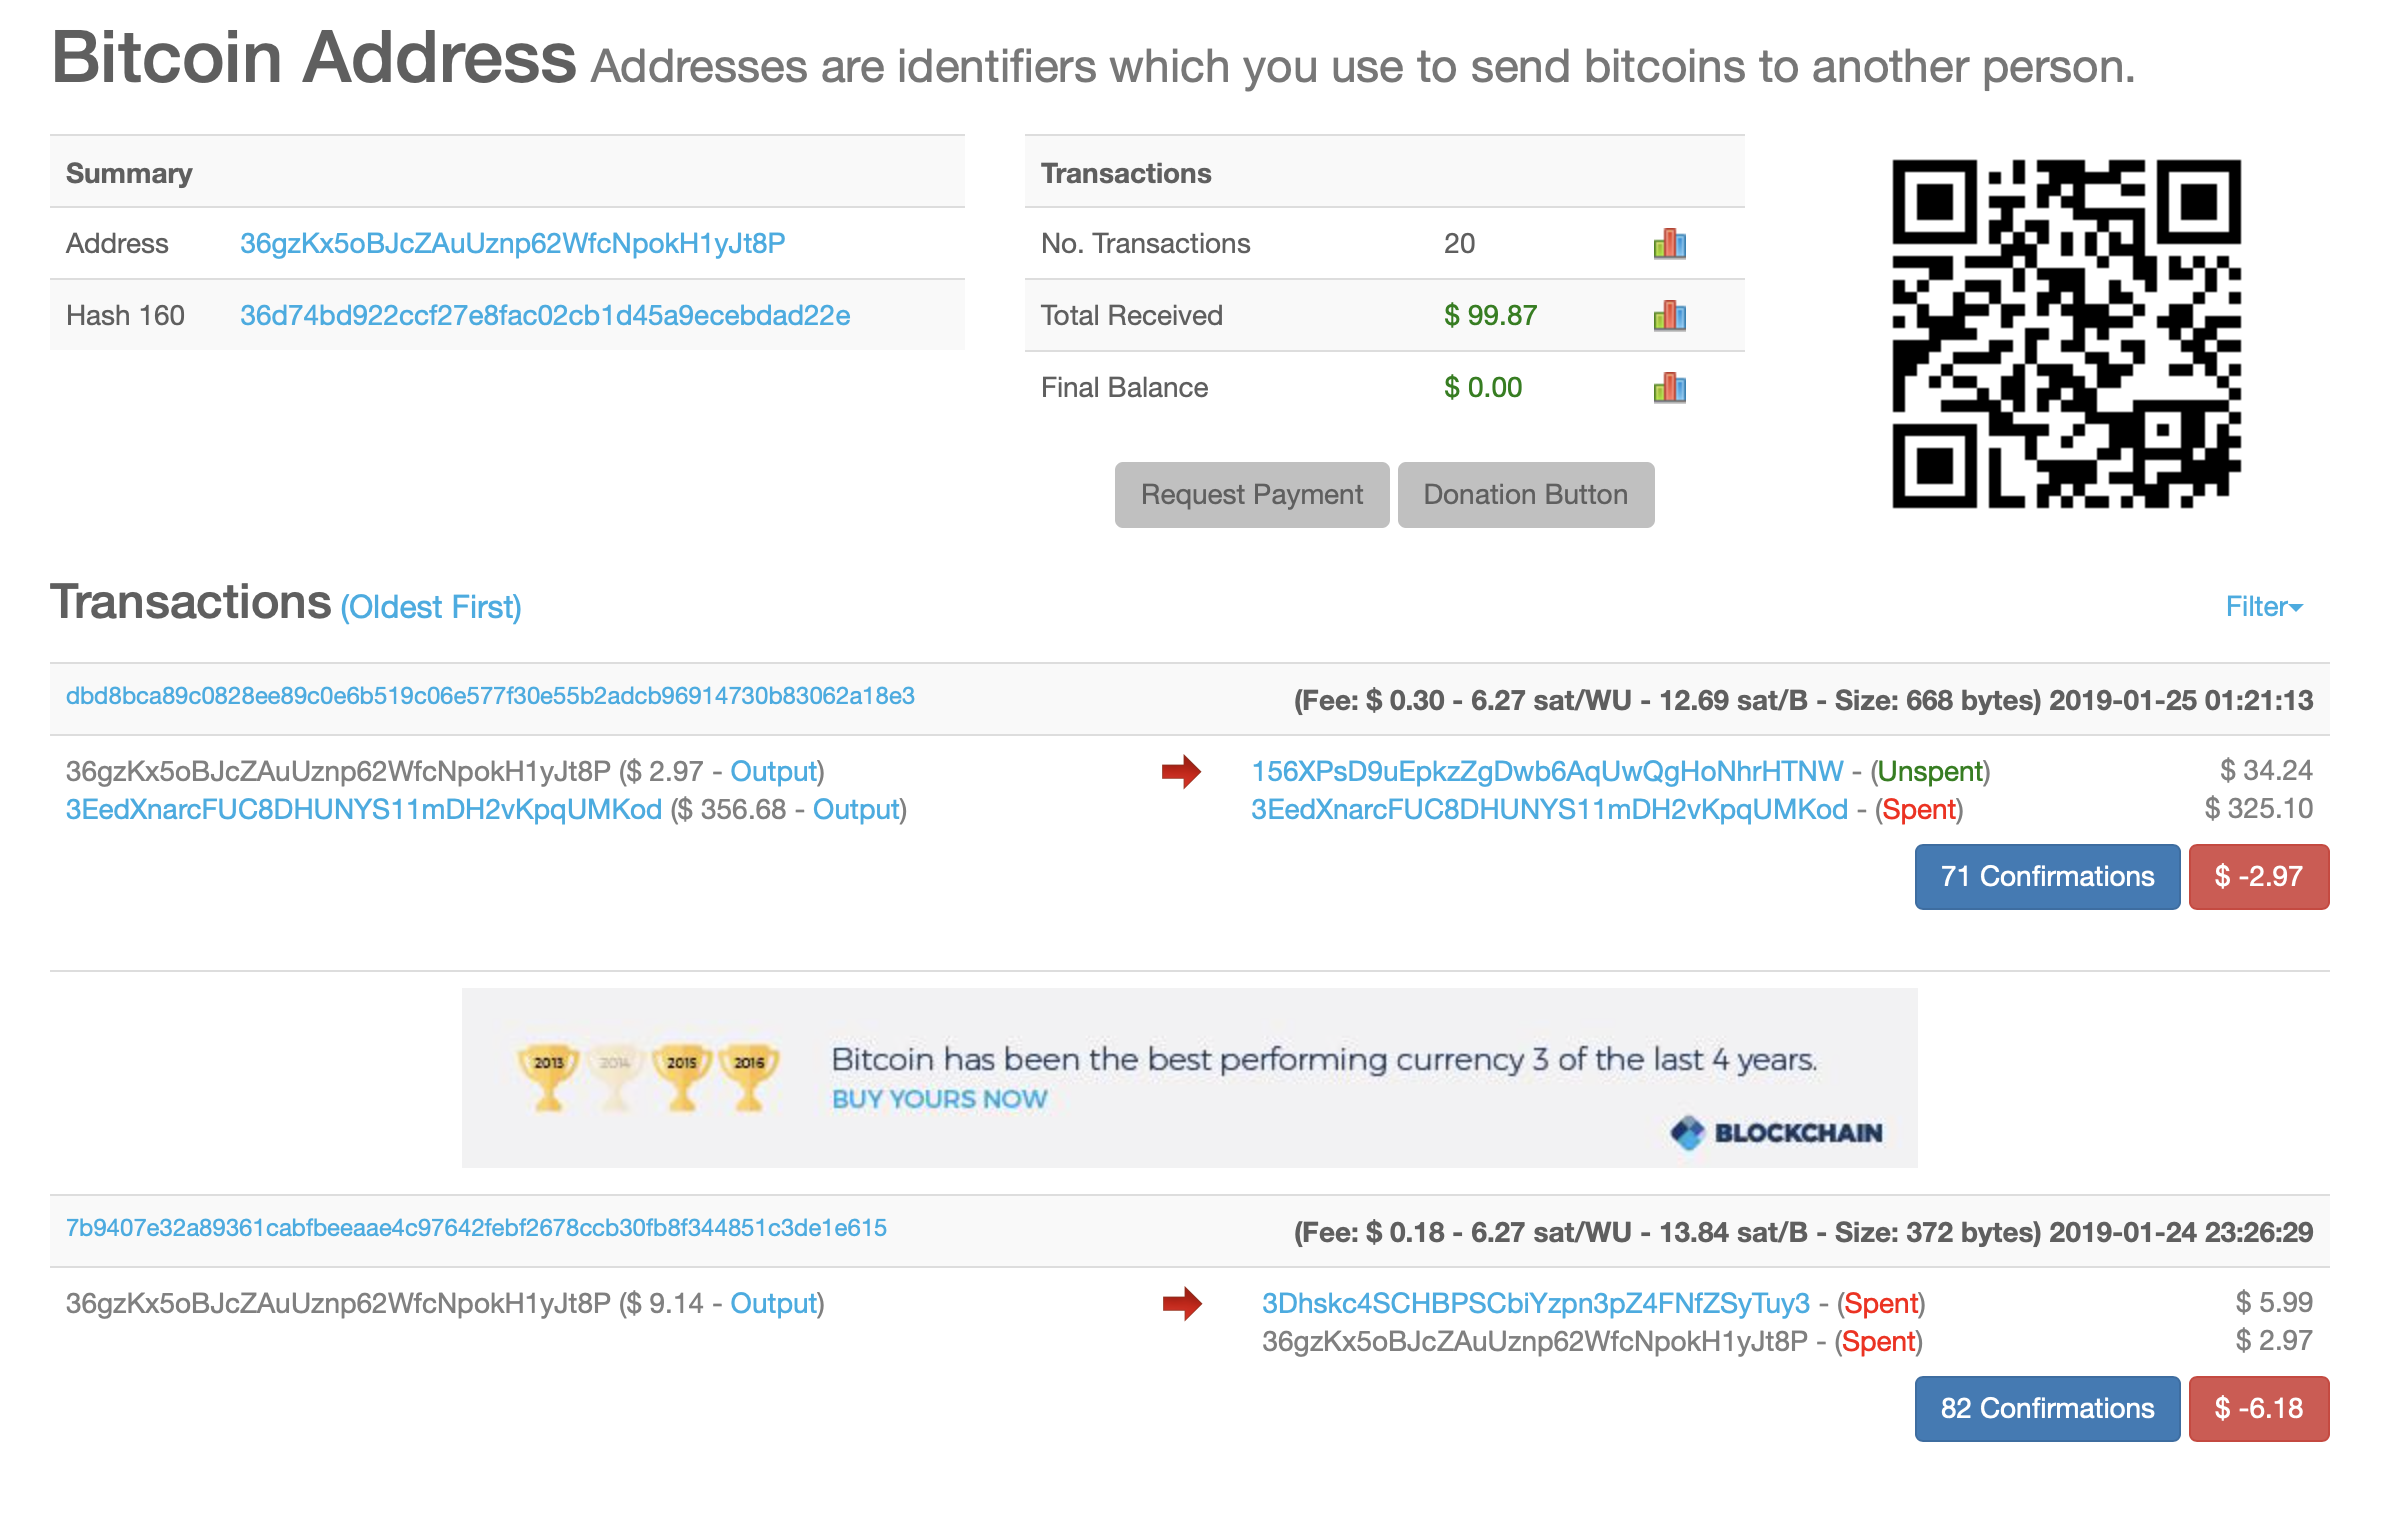
\includegraphics[width = 15cm]{./figures/chainanalysis}\\[0.5cm] 
  \caption{Blockchain Explorer's address investigation tool \cite{RefWorks:doc:5c4b1022e4b01a524cf4a1d3}.}
\end{figure}

\subsection{Chainanalysis}
Chainanalysis are a company which have built a proprietary software solution to blockchain forensics. We cannot know exactly the solutions Chainanalysis provide, or how, other than how their product is advertised. For example, for their government clients, they claim to do suspect identification, investigate criminal revenues and use pattern recognition in identifying suspicious activity. 

\subsection{Wallet Explorer}
Wallet Explorer is a website which provides similar capabilities to Blockchain Explorer in terms of inspecting addresses individually. However, Wallet Explorer additionally has a list of known entities and the public addresses they are known to be mapped to. This is extremelly useful information in understanding patterns of use and the main players in the bitcoin network, however this data is represented in quite a raw representation and is not linked with network activity, therefore on its own not extremely useful in carrying out forensic investigations.

\begin{figure}[h!]
  \centering
  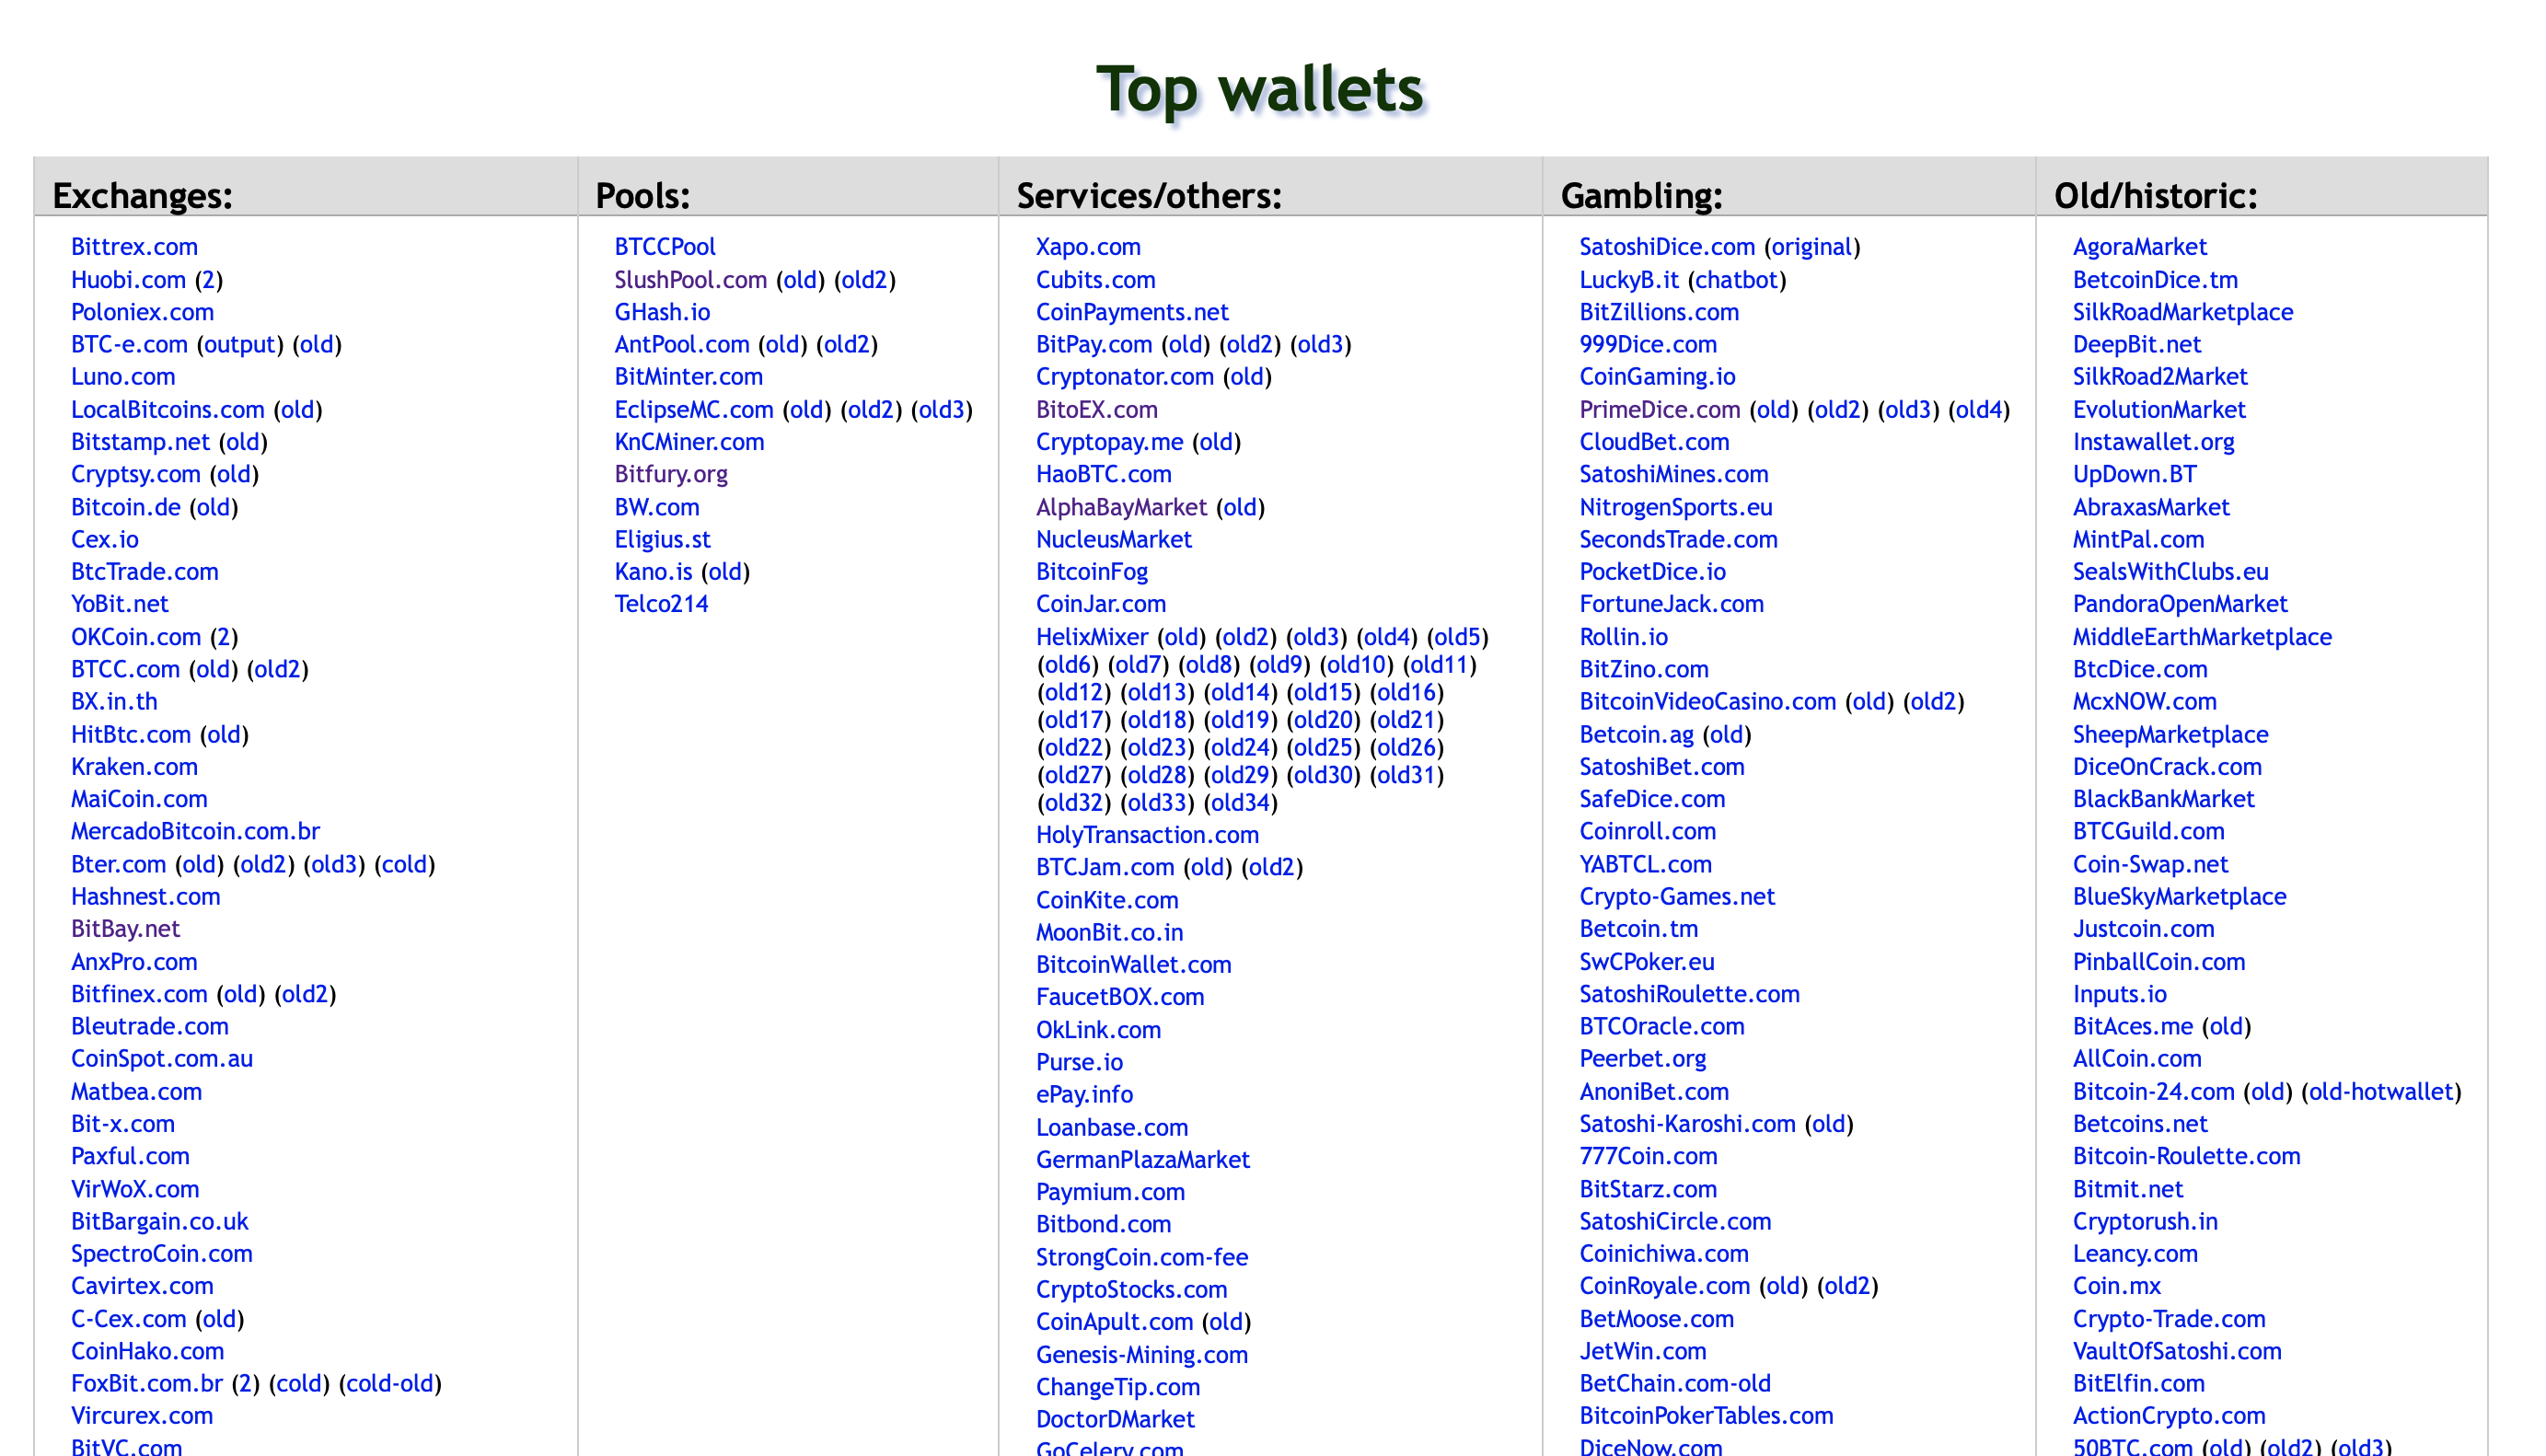
\includegraphics[width = 15cm]{./figures/walletexplorer}\\[0.5cm] 
  \caption{Wallet Explorers catalogue of wallet addresses. \cite{RefWorks:doc:5c4b26f3e4b0ea619646d513}.}
\end{figure}

\subsection{Blockpath} 
Blockpath is a website that claims to be a Bitcoin accounting tool. The feature of this site that I found the most interesting is the graphical explorer. The graph allows you to explore the relationship between addresses. However, there does not appear to be any mapping of multiple public addresses to a single entity (i.e. clustering), which would be vital to gaining real insights when performing forensic analysis.  

\begin{figure}
  \centering
  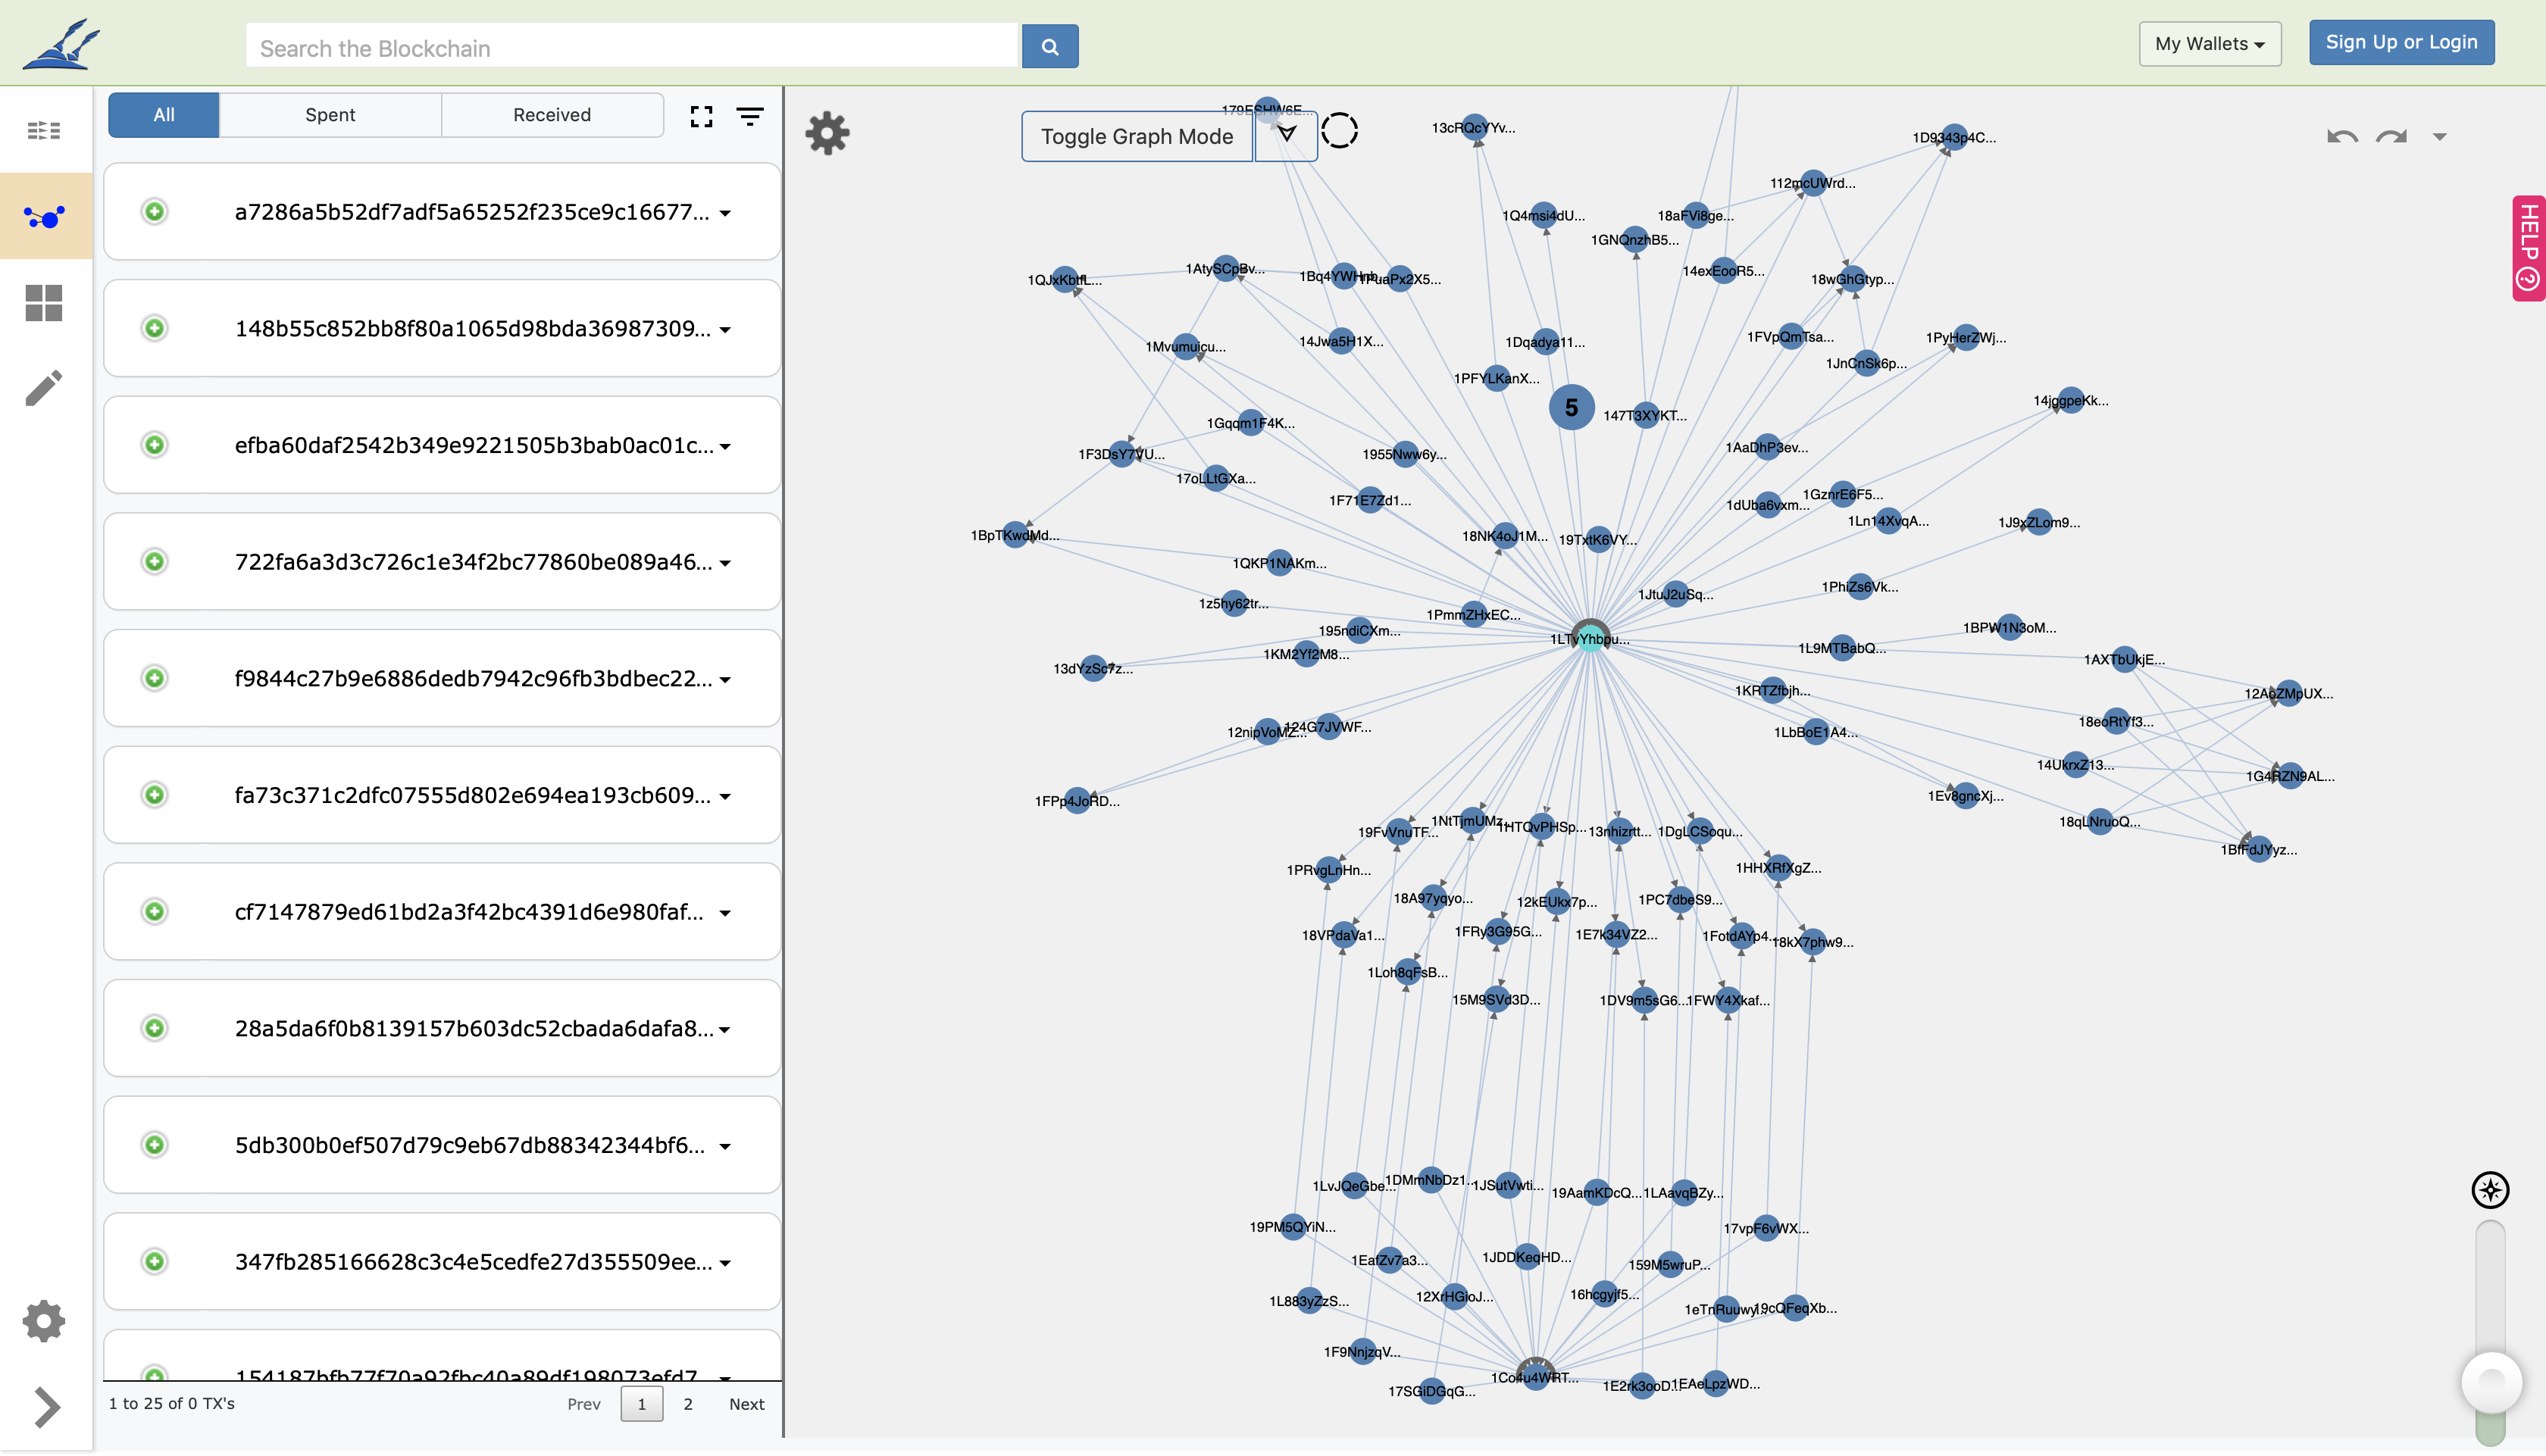
\includegraphics[width = 15cm]{./figures/blockpath}\\[0.5cm] 
  \caption{Blockpath's graphical explorer displaying transactions between addresses. \cite{RefWorks:doc:5c4b3a0ce4b0ae05280a143b}.}
\end{figure}

\subsection{Other Solutions}

There exist a number of companies claiming to offer similar solutions to Bitcoin analytics. 

\begin{itemize}
    \item \textbf{Elliptic} Similar to Chainanalysis, Elliptic offer proprietary software with main clients in finance and law enforcement. [See https://www.elliptic.co/what-we-do/bitcoin-forensics]. 
    \item \textbf{ScoreChain} Another proprietary software solution, claiming to perform Bitcoin analytics for compliance, forensics and CRM. [See https://bitcoin.scorechain.com]. 
    \item \textbf{Block Explorer:} Similar to Blockchain Explorer; providing visibility to information associated with single addresses and blocks. Also incorperates market information for many other cryptocurrencies and a cryptocurrency related news feature. [See https://blockexplorer.com/]. 

\end{itemize}


\subsection{Import Methods : Previous work}\label{design-db-previous-work}
There exists previous work in the domain of downloading the Bitcoin Blockchain. I first researched and assessed these implementations. 

\subsubsection{Bitcoin to Neo4J Tool : Open Source Project}
There exists an open source tool, built by the author of the website \url{learnmeabitcoin.com}, which populates a Neo4J database with the entire Bitcoin Blockchain \cite{RefWorks:doc:5c98e031e4b068320632cef2}. This tool requires a full Bitcoin node to be run in order to have the .dat files stored locally; the tool will parse the .dat files and write them using Cypher queries to the Neo4J database. This approach has the advantage that it is a respected approach in the community to this task and has been cited a number of times by those seeking to achieve the same goal \cite{RefWorks:doc:5c98e0cde4b044512c0b8641}; however, the tool will take several weeks (apparently 60+ days) to complete the import. 

\subsubsection{Max Baylis : Imperial MSc Project 2018}\label{background-max-baylist-project}
Max undertook a project titled 'Blockchain Data Analytics and Health Monitoring' within the Department of Computing at Imperial \cite{RefWorks:doc:5c6bd151e4b041254f892045} which involved bulk extracting data from several blockchains and writing that data to a MongoDB database. He additionally used Kafka for providing clients with the most recent blockchain updates which complimented the historical data in the database. This data was used for providing blockchain analytics in a web based environment \cite{RefWorks:doc:5c6bd151e4b041254f892045}. 

\subsubsection{TokenAnalyst : Medium Blog}
TokenAnalyst wrote a blog article on Medium with the title 'How to load Bitcoin to Neo4J in a day' \cite{RefWorks:doc:5c98e0cde4b044512c0b8641}. They describe their process of using RPC to fetch the data, writing the data to a 'data lake' in a compressed Arvo format, generating CSV's from the compressed files and feeding them to Neo4J's bulk import tool. Similar to Max's work, they then use Kafka for steaming the most recent Bitcoin data to a tool which writes it to Neo4J to keep the database up to date. 

\subsubsection{Blockchain2graph : Open Source Project}
A company Blockchain Inspector who are 'using Artificial Intelligence to fight fraud in the Blockchain' have open-sourced a tool they use with the claim that it extracts Bitcoin data and writes it to a Neo4J database \cite{RefWorks:doc:5cac6184e4b01c076c63e173}.

\subsubsection{Analysis of previous work}
TokenAnalyst's approach seems to best describe the ideal situation for this project; a efficient bulk import into Neo4J and a mechanism for keeping the database up to date. There exists no open source implementation for their work, only a high level description of what they did in their blog post. Max's work, however, is available to me and his work in fetching data using RPC could prove useful to my project. The Bitcoin to Neo4J tool would not be a feasible approach and can be immediately ruled out due to the time requirement of several weeks for the tool to complete; this would not be acceptable for the timescale of this project. As for Blockchain Inspector's open-source solution, upon inspection of the code, it seems the bulk import process relies on an existing database containing the entire Bitcoin Blockchain, and therefore seems to be more of a tool to migrate from a traditional database to a relational one (Neo4J). It is therefore not very applicable to my work, creating an intermediate database storing the Bitcoin Blockchain for the bulk import would be unnecessary and expensive.

\section{Know Your Customer}\label{background-kyc}
Know Your Customer (KYC) is a keystone in the fight against money laundering. It is the process of a business carrying out customer due-diligence measures and verify the identity of its clients. This ensures the business is deadline with bonafide customers and organisations and helps identify suspicious behaviours or practices. These measure also help satisfy anti money laundering requirements (AML). 

\section{Privacy Enhanced Crypto-currencies}
\subsection{ZCash}\label{background-zcash}
ZCash has shieldedd' transactions in which a zero knowledge proof is used to verify the sender, recipient and amount of a transaction, without exposing the information on the public blockchain. Shielded transactions are encrypted on the blockchain, yet still verified by the network using zk-SNAKRK proofs. 

\subsection{MimbleWimble (Protocol)}\label{background-mimblewimble}
MimbleWimble is a blockchain protocol which addresses gaps in many blockchain protocols by using strong cryptographic primitives to provide good scalability, privacy and fungibility. Two current implementations of the MimbleWimble Protocol are Grin and Beam. Grin is developed in Rust and is a community backed project. 

\subsection{Dash}
Dash offers a privateSend feature where users can mix the funds they are sending with others on the network; making it more difficult for a third party to identify where funds came from. There exist master nodes on the network that conduct coin mixing. 

\subsection{Monero}\label{background-monero}
Monero employs different privacy technologies to other crypto-currencies, such as Bitcoin and Ethereum which have transparent blockchains. This privacy technologies, such as ring signatures, ring confidential transactions and stealth addresses enable a verifiable blockchain but without exposing details such as the sender, recipient or the amount in a transaction. This privacy features all exist by design for all transactions; such that all transactions made with Monero are made private through these features, rather than the selective privacy provided by some other privacy enhanced crypto-currencies such as Zcash. 

\subsubsection{Kovri}
Kovri is used, a private overlay network using routing and encryption allowing users to hide their geographical location and IP address. This avoids the need to use Tor which has semi-trusted authorities, who could have overreaching influence of network consensus (and therefore in the determination of who can relay traffic). Kovri makes passive surveillance impossible. 

\subsubsection{Stealth Addresses}
Used to obscure the recipient of a transaction. Stealth addresses are one-time (ephemeral) public keys. Observers cannot infer the recipient from the stealth address, however the sender can verify that the payment was sent by then. A Monero wallet has a public view key and a public send key. When Alice sends Monero to Bob, Alice will use Bobs public view and send key, in addition to some random data in order to generate the one-time ephemeral key (stealth address). The entire blockchain can see the stealth address. Bob, with his wallet's private view key, can identify the output of the transaction sent to him on the blockchain. Bob will be able to generate a one-time private key that corresponds to the one-time public key in order to spends the funds. 

\subsubsection{Ring Signatures}
Used to obsecure the sender.
A group of possible signers of are fused together to produce a possible signature. The actual signer is a one time spend key that corresponds with an output being spent from the senders wallet; the non-signers in the ring are past transaction outputs pulled from the blockchain being used as decoys. These outputs combined make up the inputs of a transaction in which it is indistinguishable between the actual signer and the decoy signers. Key imaged are used to detect double-spends. 

\subsubsection{Ring CT signatures}
Obsecures the amount of Monero sent in a transaction. 
Before Ring CT's, Monero would require transaction amounts to be split up into smaller denominations and split amongst ring signatures to ensure there would be enough ring signers (since all signers of a ring must have outputs of the same value). This means an observer can see the amounts sent in transactions. Ring CT transactions obscure the value of outputs, but now the sender must commit to the value of an output (Pedersen commitment scheme) but without publicly disclosing the amount being sent. 




